% ------------------- Random Walk -------------------
% Google Colab - Filter Random Walk
\subsection*{Random Walk Model}
% \cite{sarkka:bayesian_filtering}

\noindent   
\textbf{State transition equation:}
\[x_t= x_{t-1} + q_{t-1}, \quad q_t \sim \mathcal{N}(0,Q)\]

\medskip
\noindent   
\textbf{Observation equation:}
$$y_t = x_t+ r_t, \quad r_t \sim \mathcal{N}(0,R)$$ 

$x_t$ is the hidden state and $y_t$ is the measurement with state transition matrix $F=1$, observation matrix $H=1$, process noise covariance $Q$ and observation noise covariance $R$.

The random walk model is one of the simplest state space models. The model assumes that the hidden state evolves over time and the observations are noisy measurements of this state. In this model, the expected state at time $t$ given the previous state is simply the same as the previous state\cmmnt{, $\mathbb{E}[x_t |x_{t-1}]=x_{t-1}$}. The model therefore describes a process with no deterministic dynamics, only random fluctuations. 

In the code $\cmmnt{Train and Test on RandomWalk.ipynb}$, the model parameters are estimated using the training dataset. The process noise variance $Q$ and and observation noise variance $R$ are fitted to maximize the likelihood of the observed data under the Kalman filter. The Kalman filter is then used to compute the filtered state means and covariances for each time step. 
An important observation from the fitted parameters is that the estimated observation noise variance $R$ is very small \cmmnt{indicating high confidence in measurements}. The model is therefore flexible enough to closely follow the observed data. 
As a consequence, the filtered estimates lie almost exactly on top of the observed values. % if we believe observation is noise free then the best estimate of the true state after seeing y_t is simply x_t


\medskip
\noindent
\textit{Formal prediction to be added!}

The predictions of the random walk are given by $\hat x_{t+1|t} = \mathbb{E}[x_{t+1|y_{1:t}}]$. Since the expected increment is zero, the predicted mean for the next state is equal to the most recent filtered estimate. This means that the distribution $p(x_{t+1}|y_{1:t})$ is centered at the current state

% Google Colab - Train and Test Filter Random Walk

\begin{figure}[H]
    \centering
    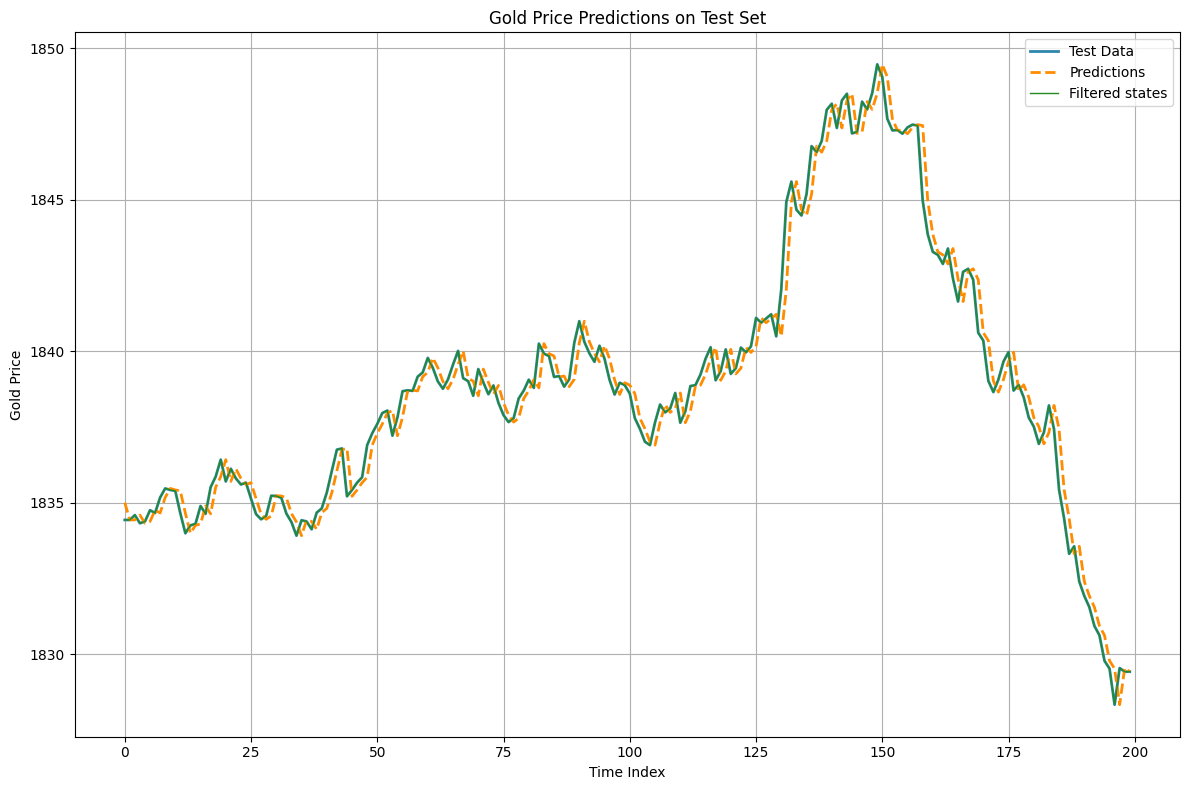
\includegraphics[width=0.5\linewidth]{Figures/Gold Price Predictions Random Walk.png}
    \caption{Gold price predictions on test set with random walk}
    \label{fig:randwal}
\end{figure}

In Figure \ref{fig:randwal}, we observe that the filtered states follow the observations almost same. This is expected because the estimated observation noise is very small. On the other hand, the predicted values are slightly shifted from the true observations because the model uses the current filtered estimate as its best guess for the next state. 

The predictions would appear more random if the process noise covariance $Q$ were increased. \cmmnt{Filtering estimates the state given the current observation after having seen it so it can almost exactly match the observed data when $R$ is small. Prediction estimates the state for the next time step before seeing the observation, so it cannot adjust to new data and reflects only the model's prior dynamics.}




\newpage
% ------------------- Linear Growth Model/ Local Linear Trend State Space Model -------------------
% \cite{triantafyllopoulos:bayesian_state_space}
\subsection*{Local Linear Trend Model}

\medskip
\noindent 
\textbf{State vector:}
\[x_t= \begin{bmatrix} 
                \ell_t \\ 
                \mu_t 
            \end{bmatrix}\]

where $\ell_t$ is the local level and $\mu_t$ is the local slope.

\medskip
\noindent
\textbf{State transition equation:}
$$x_{t+1} = Fx_t + q_t$$ 

with transition matrix
$F=\begin{bmatrix} 
        1 & 1 \\ 
        0 & 1
    \end{bmatrix},$
$q_t = \begin{bmatrix}
    \eta_t \\ \zeta_t
\end{bmatrix}$
and process noise covariance
$Q=\begin{bmatrix} 
        \sigma^2_\eta & 0 \\ 
        0 & \sigma^2_\zeta 
    \end{bmatrix}.$

\medskip
\noindent     
\textbf{Observation equation:}
$$y_t = Hx_t+\epsilon_t, \quad \epsilon_t \sim \mathcal{N}(0, \sigma^2_\epsilon)$$ 

with the observation matrix \[H=\begin{bmatrix} 1 & 0 \end{bmatrix}.\]

\begin{itemize}
    \item $\eta_t$ level noise, 
    \item $\zeta_t$ slope noise and
    \item $\epsilon_t$ observation noise. 
    \item $\mu_t$ follows a linear function and a random error $\zeta_t$
\end{itemize}

\medskip
\noindent 
\textbf{Component form:}
% component form shows the individual dynamics of y_t and \beta_t whereas matrix form is compact and convenient for algorithms (Kalman filter, smoothing)
\begin{align*}
    % level: previous level + slope + random noise \eta_t
    \ell_{t+1} &= \ell_t + \mu_t + \eta_t, &\eta_t \sim \mathcal{N}(0, \sigma^2_\eta)\\
    % slope: random walk + noise \zeta_t
    \mu_{t+1} &= \mu_t + \zeta_t, &\zeta_t \sim \mathcal{N}(0, \sigma^2_\zeta)\\
    % observation equation 
    y_t &= \ell_t+\epsilon_t, &\epsilon_t \sim \mathcal{N}(0, \sigma^2_\epsilon)
\end{align*}


\medskip
The local linear trend model is an extension of the random walk that introduces a trend component to capture local slopes \cmmnt{or drifts} in the data over time. The state vector consists of two elements, the local level $\ell_t$ and the local slope $\mu_t$. $Q$ is the process noise covariance for the level and trend components. While the random walk assumes that the expected change of the state is zero, the local linear trend model allows for a time-varying mean change determined by $\mu_t$. Again, in the code \cmmnt{Train and Test von FilterLocalLinearTrendModel.ipynb}, the model parameters are estimated using the training dataset. The process and observation noise variances are fitted by maximizing the likelihood under the Kalman filter. The filter then computes the filtered state means and covariances at each time step. The filtered level follows the data closely, while the estimated trend captures the local direction of the change. 

\medskip
\noindent
\textit{Formal prediction to be added!}


\begin{figure}[H]
    \centering
    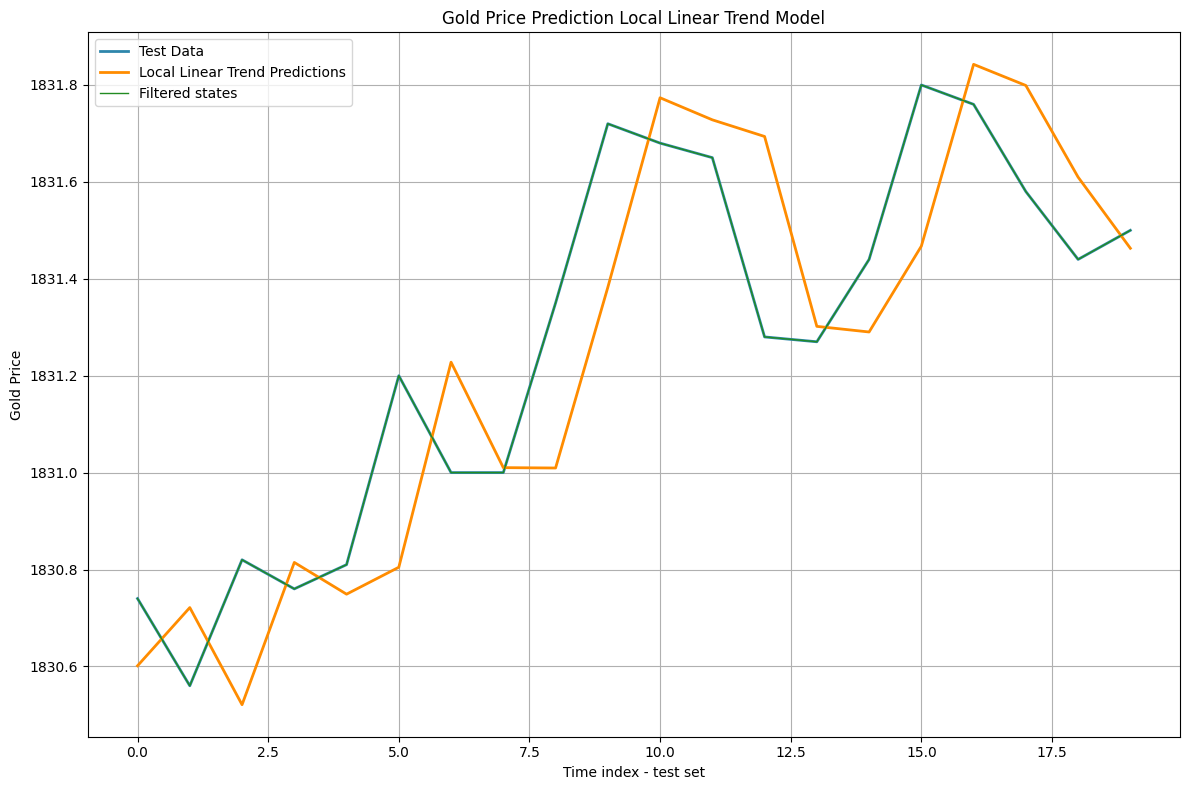
\includegraphics[width=0.5\linewidth]{Figures/Gold Price Predictions Local Linear Trend Model.png}
    \caption{Gold price predictions on test Set with local linear trend model}
    \label{fig:loclin}
\end{figure}

In Figure \ref{fig:loclin}, we again observe that the filtered state follows the observation in a nearly identical manner. This is also expected because the estimated observation noise is very small. However, the predicted values are slightly shifted relative to the observations because the model uses the current filtered estimate as its best guess for the next state. 

If the process noise covariance $Q$ were increased, the prediction would appear more random. 


% -----------------------------------------------------------
% Color Scheme:
% 1. Actual Data: '#2E86AB' 
% 2. Predictions: 'darkorange' 
% 3. Filtered States: 'forestgreen' 
% 4. Prediction Errors: 'purple' 
% 5. Filtered Errors: 'red' 
% 6. Zero Line: 'gray' 

% Consistent Sizing:
% 1.  All figures use $FIG_SIZE = (12, 8)$ for uniformity

% Enhanced Analysis:
% - Shows both prediction errors AND filtered state errors
% - Comprehensive performance metrics
% - Clear distinction between different types of estimates
